%%%%%%%%%%%%%%%%%%%% manuscript.tex %%%%%%%%%%%%%%%%%%%%%%%%%%%%%%%%%%%
%
% Springer proceedings template (svproc class)
% Content: CARLA-MAMBA for time-series anomaly detection
%
%%%%%%%%%%%%%%%% Springer %%%%%%%%%%%%%%%%%%%%%%%%%%%%%%%%%%

\documentclass[runningheads]{llncs}
\usepackage[T1]{fontenc}

\usepackage{graphicx}
\usepackage{caption}
\usepackage{subcaption}
\usepackage{float}

\usepackage{booktabs}

\usepackage{multirow}

\usepackage{array}

\usepackage{xurl}

\usepackage{amssymb}  
\usepackage{amsmath}
\usepackage{makecell}

\usepackage[hidelinks]{hyperref}
\raggedbottom
\setlength{\emergencystretch}{2em}
\begin{document}
\title{A Framework for Time-Series Anomaly Detection with Mamba Backbone}

\titlerunning{A Framework for Time-Series Anomaly Detection}

%\author{Lam Huynh Khang\inst{3}, Vo Thi Ngoc Chau\inst{1,2} \and  Tri Minh Pham\inst{1,2,3}}

%\authorrunning{Lam et al.}

%\institute{Ho Chi Minh City University of Technology(HCMUT) 
%\and Vietnam National University, Ho Chi Minh City, Vietnam
%\and AiTA Lab, Faculty of Information Technology, FPT University
%\email khanglhse200666@fpt.edu.vn ,chauvtn@hcmut.edu.vn, tri.phamhpc@hcmut.edu.vn}
\maketitle
\begin{abstract}
Time-series anomaly detection is an important problem in many real-world systems such as industrial monitoring and cloud infrastructure. CARLA is a strong self-supervised framework for this task, but it uses a ResNet backbone in the pretext stage, which has limited ability to model long-range temporal patterns. In this paper, we propose CARLA-MAMBA, which replaces the ResNet backbone in the pretext stage with Mamba, a selective state space model that can process long sequences efficiently. Mamba captures temporal dependencies better than ResNet while keeping computation fast. We conduct systematic window size ablation experiments across seven benchmark datasets and find that the optimal window size is governed by two interacting factors: the mean series length and the hardware memory budget. We show that CARLA-MAMBA with properly tuned window sizes substantially outperforms the original CARLA baseline on all datasets. Our results suggest that Mamba is a good choice of backbone for self-supervised time-series anomaly detection.
\keywords{time-series, anomaly detection, contrastive learning, Mamba, state space model, self-supervised learning, window size selection}
\end{abstract}

% ---- Introduction ----
\section{Introduction}
\label{sec:introduction}

Time-series anomaly detection has become a critical component in many real-world systems, including industrial monitoring, cloud infrastructure, and cyber-physical environments. In these applications, the ability to accurately identify rare and abnormal patterns is essential for maintaining system reliability and preventing failures. However, this task remains challenging due to the inherent characteristics of time-series data, such as long temporal dependencies, high dimensionality, and, most importantly, the lack of labeled data in practical scenarios \cite{darban2022deep}. As a result, many recent studies have focused on unsupervised and self-supervised approaches that aim to learn representations of normal behavior without relying on explicit annotations.

Among these approaches, CARLA \cite{darban2024carla} has emerged as a strong self-supervised framework for time-series anomaly detection. It adopts a two-stage learning strategy, where the first stage focuses on contrastive representation learning through a pretext task, and the second stage performs self-supervised classification based on neighborhood relationships in the learned feature space. By taking advantage of anomaly injection and contrastive objectives, CARLA is able to learn discriminative representations that separate normal and anomalous patterns effectively. Despite its strong performance, CARLA relies on a ResNet backbone \cite{fawaz2019deep} in both stages, which was originally designed for image data. While convolutional architectures are effective at capturing local patterns, they do not explicitly model temporal order, limiting their ability to capture long-range dependencies that are essential in time-series data.

Recent advances in sequence modeling have highlighted the importance of architectures that can better capture long-range temporal relationships while maintaining computational efficiency. In particular, state space models (SSMs) have gained attention as a promising alternative to traditional convolutional and attention-based approaches. These models provide a principled framework for modeling sequential data through latent states and have demonstrated strong performance on long-sequence tasks with linear computational complexity \cite{gu2022efficiently}. Mamba \cite{gu2023mamba} is among the best because it possesses a selective mechanism that allows the model to dynamically control the flow of information at each time step. This enables more effective modeling of temporal dependencies compared to fixed-kernel architectures, while also maintaining efficient training and inference.

Motivated by these observations, this paper proposes CARLA-MAMBA, a modified version of the CARLA framework in which the ResNet backbone in the pretext stage is replaced with a Mamba-based encoder. Figure~\ref{fig:carla_resnet} illustrates the original CARLA architecture using ResNet in both stages, while Figure~\ref{fig:carla_mamba} shows the proposed CARLA-MAMBA framework where the pretext encoder is replaced by Mamba. The rest of the pipeline, including the anomaly injection strategy and the self-supervised classification stage, is preserved to ensure a fair comparison. By introducing a sequence-aware backbone into the representation learning stage, the proposed method aims to improve the quality of learned features and enhance anomaly detection performance.

We evaluate the proposed approach on seven widely used benchmark datasets, including MSL, SMAP, SMD, SWaT, WADI, Yahoo-A1, and KPI \cite{hundman2018detecting,su2019robust,mathur2016swat,ahmed2017wadi,laptev2015benchmark}. The key contribution of this work is a systematic window size ablation study across all datasets, from which we derive a practical two-factor heuristic for window size selection based on mean series length and GPU memory constraints. Experimental results show that CARLA-MAMBA with properly selected window sizes substantially outperforms the original CARLA baseline across all seven datasets.

In summary, this work makes the following contributions. First, we introduce a Mamba-based encoder into the CARLA framework to better capture temporal dependencies in time-series data. Second, we conduct extensive window size ablation experiments on multiple benchmark datasets and derive a practical heuristic for window size selection. Finally, we provide a comprehensive analysis of performance, efficiency, and resource usage, offering insights into the trade-offs between different backbone architectures.

The source code for CARLA-MAMBA is publicly available at 
\url{https://github.com/Welkie/mamba_carla}.

% ---- Related Work ----
\section{Related Work}

\subsection{Time Series Anomaly Detection}
\label{sec:related_tsad}

The detection of anomalies within time series data has been the subject of extensive research, using an array of techniques from statistical methods to classical machine learning and, more recently, deep learning models \cite{schmidl2022anomaly}. Established statistical techniques such as moving averages like the ARIMA model \cite{box1970distribution} have seen widespread application. Machine learning techniques, including clustering algorithms and density-based approaches, alongside algorithms similar to decision trees \cite{liu2008isolation} have also been leveraged.

Deep Learning methods in TSAD: In recent years, deep learning has proven highly effective due to its ability to autonomously extract features \cite{pang2021deep}. The focus within TSAD is largely on unsupervised \cite{hundman2018detecting}, semi-supervised \cite{park2018multimodal}, and recently self-supervised \cite{yue2022ts2vec} approaches, addressing the issue of scarce labelled data. Deep learning techniques, encompassing autoencoders \cite{yao2023regularizing}, variational autoencoders (VAEs) \cite{park2018multimodal}, RNNs \cite{su2019robust}, LSTM networks \cite{hundman2018detecting}, and Transformers \cite{tuli2022tranad,xu2021anomaly} have shown potential in TSAD.

\subsection{Contrastive Learning for Time Series}

Contrastive representation learning has been successful in image analysis \cite{chen2020simple} and natural language processing \cite{logeswaran2018efficient}, and its use in TSAD has grown recently. TS2Vec \cite{yue2022ts2vec} learns multi-level representations using a hierarchical contrastive approach. DCdetector \cite{yang2023dcdetector} uses dual attention with contrastive loss. CARLA \cite{darban2024carla} is a more recent framework that uses anomaly injection and neighbor-based classification to improve detection accuracy, and achieves state-of-the-art results on seven benchmark datasets.

\subsection{State Space Models and Mamba}

Structured state space sequence models (SSMs) are a class of deep learning models that model sequences through a latent state \cite{gu2022efficiently}. S4 \cite{gu2022efficiently} was one of the first SSMs to show strong performance on long-sequence benchmarks. Later work such as S5 \cite{smith2023simplified} improved efficiency further.

Mamba \cite{gu2023mamba} extends prior SSMs by adding a selection mechanism. Unlike earlier SSMs that are linear time-invariant (LTI), Mamba allows its parameters to change based on the input. This means the model can selectively keep or ignore information at each time step. Mamba also uses a hardware-aware parallel scan algorithm that keeps training and inference fast even for very long sequences. These properties make Mamba well-suited for time-series data, where important patterns can appear across long temporal ranges. 

More recent studies have explored Mamba-based architectures for time-series modeling and anomaly detection. Xu et al.~\cite{xu2024sst} proposed a hybrid Mamba-Transformer architecture that assigns Mamba to long-range pattern modeling and Transformer to short-range dynamics, achieving strong forecasting performance with linear complexity. Chen et al.~\cite{chen2024joint} demonstrated that combining selective state space modeling with detrending yields robust anomaly detection across multiple benchmarks. Sellam et al.~\cite{sellam2025maat} further explored hybrid Mamba-Transformer mechanisms for time-series anomaly detection, improving anomaly representation and localization in complex industrial datasets.

\subsection{Window Size Selection in Time Series Models}
 
Window size is a fundamental hyperparameter in sliding-window-based time-series models that directly affects the temporal context available to the encoder. Prior work in time series classification suggests that window size should roughly match the characteristic period or anomaly duration of the signal \cite{fawaz2019deep}. In practice, however, this quantity is rarely known in advance, and practitioners typically rely on grid search or dataset-specific heuristics. In the context of Mamba-based models, window size has an additional effect on GPU memory consumption, since the Mamba state is maintained across the full sequence length. This interaction between sequence modeling capacity and hardware constraints is underexplored in prior work and motivates our systematic ablation study.

% ---- Materials and Methods ----
\section{Materials and Methods}

\subsection{Baseline Framework: CARLA}

CARLA \cite{darban2024carla} is a two-stage self-supervised deep learning framework designed for anomaly detection in time series data. It does not need ground-truth labels and learns to detect anomalies by understanding normal behaviors.

In the first stage (pretext stage), the input time series is divided into fixed-length windows using a sliding window approach. Each window is encoded by a ResNet-based feature extractor followed by an MLP projection head. The model is trained using a triplet contrastive loss. For each anchor window $w_i$, a positive sample is a nearby window in time, and a negative sample is a version of $w_i$ with an injected synthetic anomaly. The loss function is:
\begin{equation}
\mathcal{L}_{\text{Pretext}}(\phi_p, \mathcal{T}, \alpha) = \frac{1}{|\mathcal{T}|} \sum_{(a,p,n) \in \mathcal{T}} \max(\|\phi_p(a) - \phi_p(p)\|_2^2 - \|\phi_p(a) - \phi_p(n)\|_2^2 + \alpha,\ 0)
\end{equation}
where $a$, $p$, and $n$ denote the anchor, positive, and negative windows, respectively. 
$\mathcal{T}$ represents the set of all triplets used during training. 
$\phi_p(\cdot)$ is the encoder network that maps an input window into the latent embedding space, and $\alpha$ is the margin hyperparameter that enforces separation between positive and negative pairs. 
The term $\|\phi_p(a)-\phi_p(p)\|_2^2$ minimizes the distance between temporally related windows, while $\|\phi_p(a)-\phi_p(n)\|_2^2$ increases the distance between normal and anomaly-injected windows.

After training, for each window in the training set, the model finds its $Q$ nearest neighbors and $Q$ furthest neighbors in the embedding space. These neighbor sets are used as input to the second stage.

In the second stage (self-supervised classification), a classifier $\phi_s$ is initialized from the pretrained encoder $\phi_p$. It is trained using a loss that pushes each window toward its nearest neighbors and away from its furthest neighbors in class space:
\begin{equation}
\mathcal{L}_{\text{SS}} = \mathcal{L}_{\text{consistency}} - \mathcal{L}_{\text{inconsistency}} - \beta \cdot \mathcal{L}_{\text{entropy}}
\end{equation}
where $\mathcal{L}_{\text{consistency}}$ encourages windows and their nearest neighbors to share similar class predictions, 
$\mathcal{L}_{\text{inconsistency}}$ separates windows from their furthest neighbors in the embedding space, 
and $\mathcal{L}_{\text{entropy}}$ is an entropy regularization term that prevents trivial class assignments. 
The coefficient $\beta$ controls the contribution of the entropy regularization term.

At inference time, the majority class in the training set is treated as normal. A test window is flagged as anomalous if it is not assigned to the majority class.

In the original CARLA, both stages use a 3-layer ResNet with kernel sizes $[8, 5, 3]$ and representation dimension 128. ResNet extracts local features well, but it was designed for images and does not explicitly model the order of time steps.

\subsection{Proposed Method: CARLA-MAMBA}

We propose CARLA-MAMBA, where the ResNet backbone in the pretext stage is replaced with a Mamba encoder. The anomaly injection strategy, neighbor search, and the classification stage all remain the same as in the original CARLA \cite{darban2024carla}.

\subsubsection{Mamba as a Sequence Encoder}

Mamba \cite{gu2023mamba} is a selective state space model (SSM). The core SSM equations are:
\begin{align}
h'(t) &= \mathbf{A}h(t) + \mathbf{B}x(t) \\
y(t) &= \mathbf{C}h(t)
\end{align}
where $h(t)$ is the hidden state, and $\mathbf{A}$, $\mathbf{B}$, $\mathbf{C}$ are the system parameters. The continuous system is first discretized using a time step $\Delta$, then computed as a recurrence or convolution.

In Mamba, the parameters $\mathbf{B}$, $\mathbf{C}$, and $\Delta$ depend on the current input $x$. This allows the model to decide at each step how much of the current input to absorb into the state, and how much of the previous state to keep. This selective behavior helps the model focus on relevant parts of the sequence and ignore noise.

Mamba also uses a hardware-aware parallel scan algorithm to avoid the slow sequential computation of recurrent models. It keeps intermediate states in fast GPU memory (SRAM) instead of slow memory (HBM), which greatly reduces the time needed \cite{gu2023mamba}.

\subsubsection{Integration into CARLA}

In CARLA-MAMBA, an input window $\{x_t\}_{t=1}^{T}$ is processed by the Mamba encoder to produce a feature vector. 
The resulting vector is then passed to an MLP projection head, 
which outputs the final embedding for the contrastive loss.

Only the pretext stage encoder is changed. The self-supervised classification stage still uses a ResNet backbone, as in the original CARLA. Because Mamba and ResNet have different architectures, the backbone weights from the pretext stage cannot be directly transferred to the classification stage. Instead, the main benefit of using Mamba in the pretext stage comes from the quality of the neighbor sets. After pretext training, each window's nearest and furthest neighbors are computed based on the Mamba embeddings. These neighbor sets are then used as input to the classification stage. Therefore, better representations from Mamba lead to more accurate neighbor assignments, which in turn help the classification stage learn better decision boundaries.

We choose to replace only the pretext stage because this stage determines the quality of the learned representations and the resulting neighbor structure. Since the downstream classification stage relies directly on these learned embeddings, modifying the pretext encoder is sufficient to evaluate the impact of Mamba on representation learning and anomaly detection performance.

\begin{figure}[H]
    \centering
    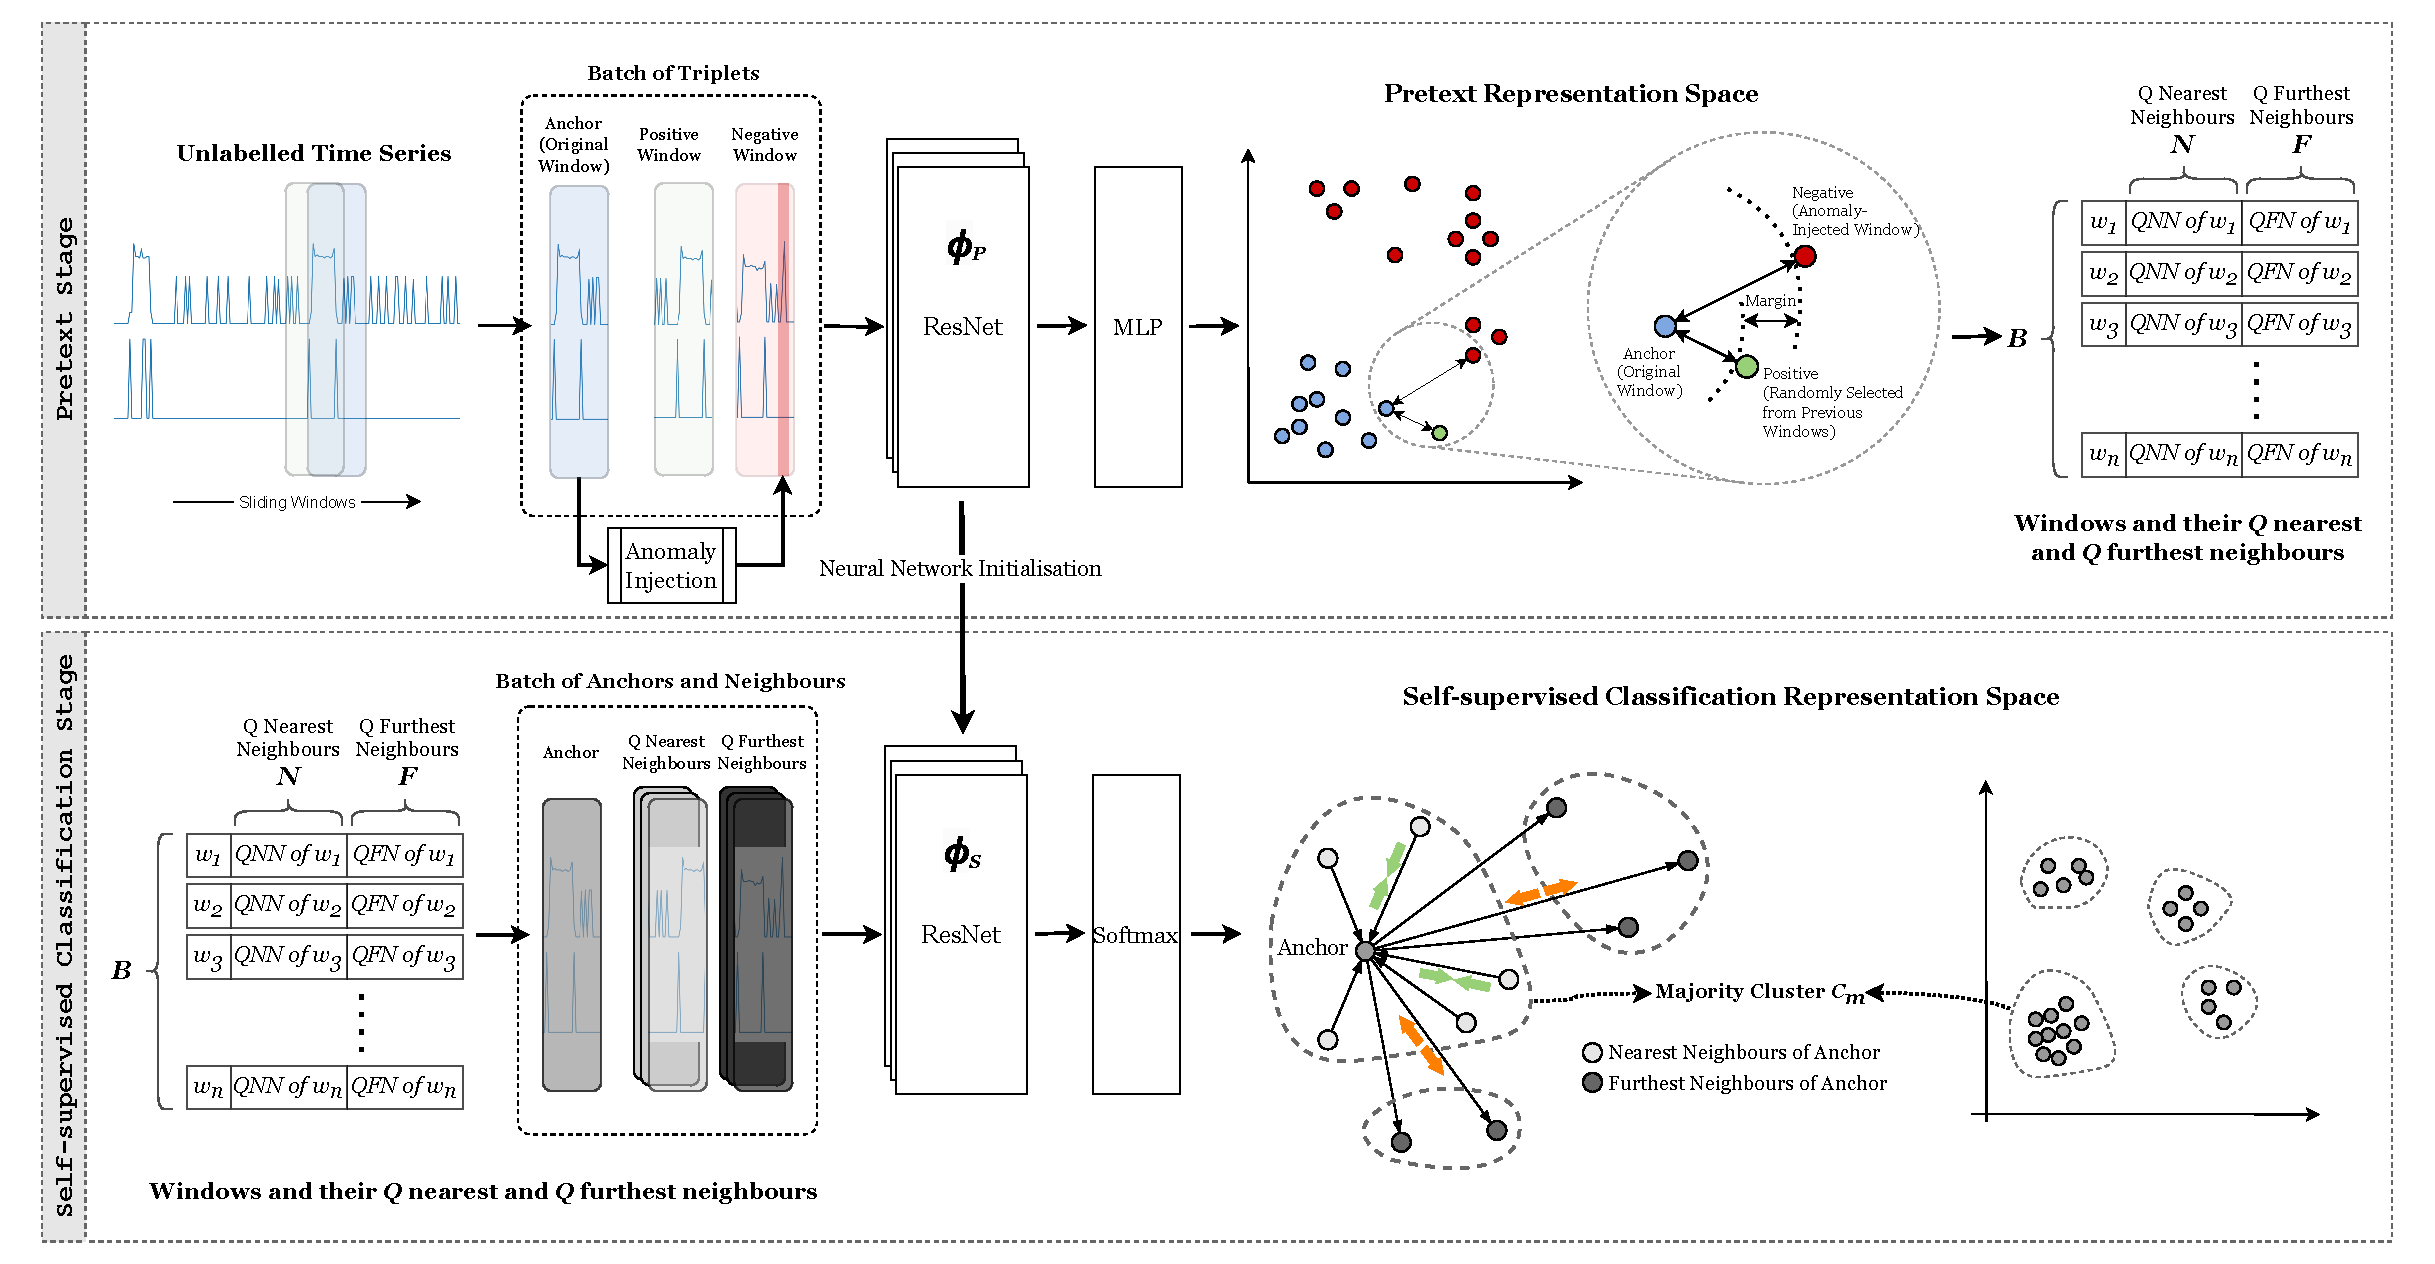
\includegraphics[
        width=0.92\linewidth,
        height=0.38\textheight,
        keepaspectratio
    ]{images/figure1_a}
    \caption{Original CARLA architecture with ResNet backbone in both stages \cite{darban2024carla}.}
    \label{fig:carla_resnet}
\end{figure}

\begin{figure}[H]
    \centering
    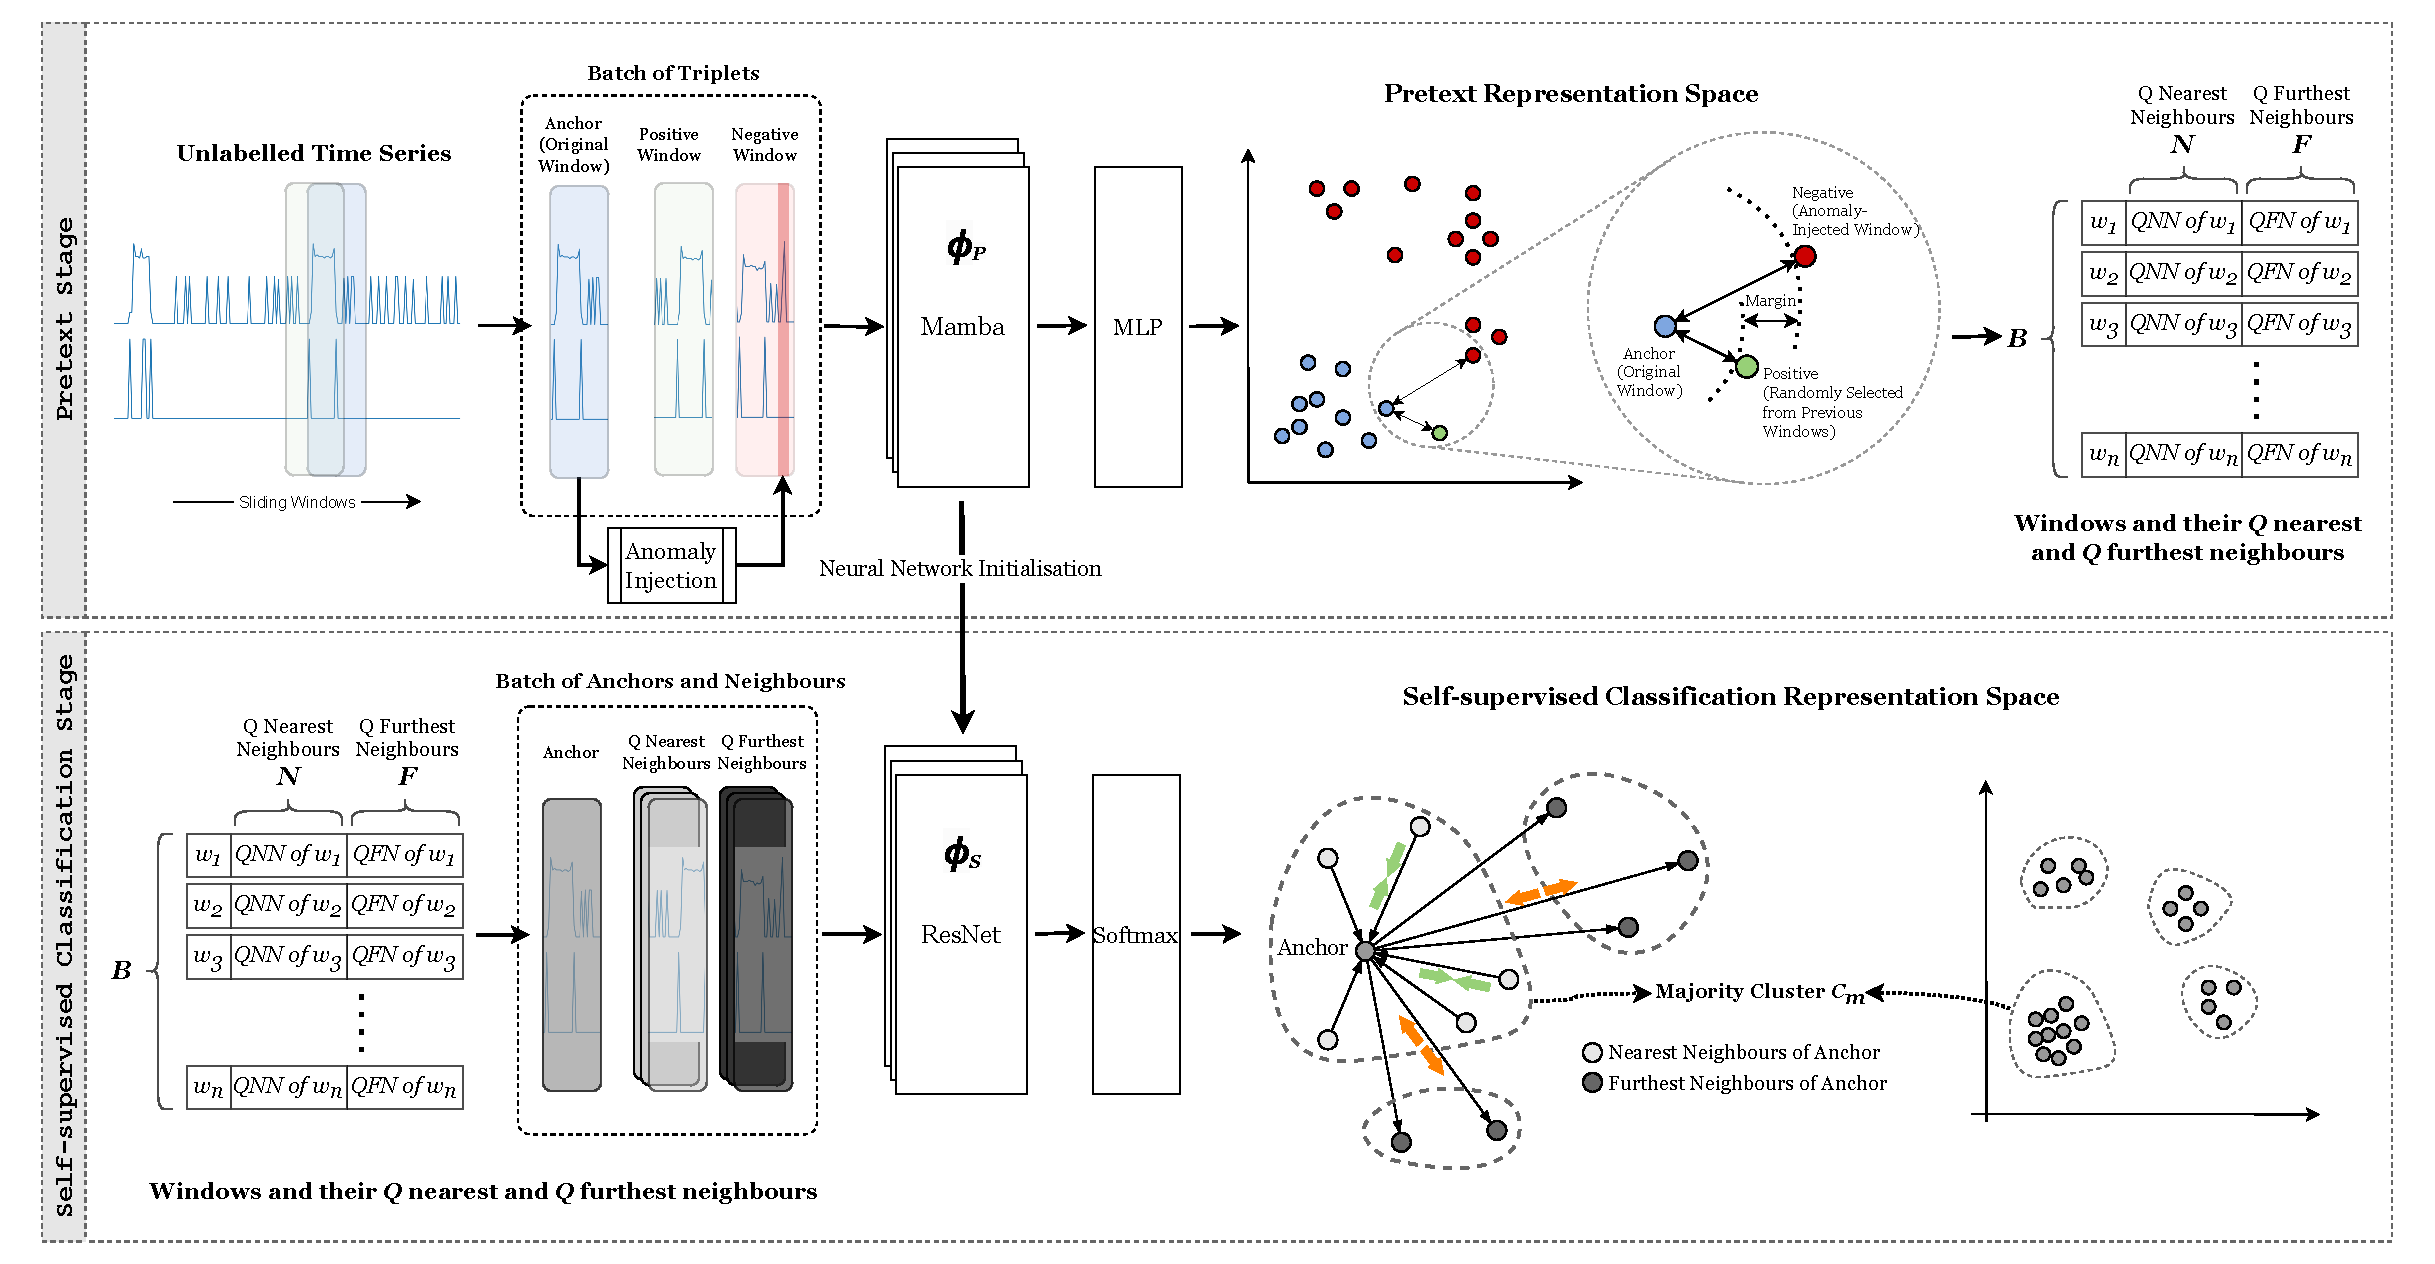
\includegraphics[
        width=0.92\linewidth,
        height=0.38\textheight,
        keepaspectratio
    ]{images/figure1_c}
    \caption{CARLA-MAMBA replaces the ResNet encoder in the pretext stage only.}
    \label{fig:carla_mamba}
\end{figure}

\subsection{Datasets}

We evaluate our method on seven widely used benchmark datasets for time-series anomaly detection. The detailed statistics of all datasets are summarized in Table~\ref{tab:datasets}. These datasets cover diverse characteristics, including multivariate and univariate time series, different anomaly ratios, and multiple application domains such as spacecraft monitoring, industrial systems, and web services.
\begin{table}[htbp]
\centering
\caption{Summary of benchmark datasets used in our experiments.}
\label{tab:datasets}
%\resizebox{\linewidth}{!}{
\begin{tabular}{lcccccc}
%\hline
\toprule
\textbf{Dataset} & \textbf{\#Series} & \textbf{Dims} & \textbf{Train Size} & \textbf{Test Size} & \textbf{Anomaly (\%)} & \textbf{Ref} \\
\midrule
MSL      & 27 & 55  & 58,317  & 73,729  & 10.53 & \cite{msl_smap_dataset} \\
SMAP     & 55 & 25  & 140,825 & 444,035 & 12.85 & \cite{msl_smap_dataset} \\
SMD      & 28 & 38  & 708,405 & 708,420 & 4.16  & \cite{smd_dataset} \\
SWaT     & 1  & 51  & 496,800 & 449,919 & 12.14 & \cite{swat_dataset_kaggle} \\
WADI     & 1  & 123 & 784,568 & 172,801 & 5.77  & \cite{wadi_dataset_kaggle} \\
Yahoo-A1 & 55 & 1   & 39,096  & 39,136  & 3.79  & \cite{yahoo_a1_dataset} \\
KPI      & 29 & 1   & 1,459,418 & 1,459,429 & 2.21 & \cite{kpi_dataset} \\
\bottomrule
\end{tabular}
%}
\vspace{-5pt}
\end{table}
All datasets are publicly available and have been widely used in prior research. The train, test splits follow the original CARLA protocol, and no additional preprocessing is applied.

\subsection{Training Protocol}
 
To ensure a fair and reproducible comparison, all experiments are conducted on a single NVIDIA Tesla T4 GPU with 16~GB of memory. CARLA-ResNet uses the window sizes selected by the original authors \cite{darban2024carla} (200 for MSL, SMAP, SMD, SWaT; 400 for WADI; 250 for Yahoo-A1 and KPI). For CARLA-MAMBA, the best-performing window size from the ablation study is used as the final configuration for reporting results.
 
For training epochs, SWaT and WADI use 10 pretext epochs while the other datasets use 30. This is because SWaT and WADI are large single-series datasets that require more time per epoch, and the T4 GPU session time is limited. The same number of epochs is used for both variants on each dataset.
 
Table~\ref{tab:hyperparams} summarizes the key hyperparameters used in the final comparison.
 
\noindent
\begin{minipage}{\linewidth}
\centering

\captionsetup{type=table}
\caption{Hyperparameter settings for CARLA-ResNet and CARLA-MAMBA (final configuration). Window sizes for CARLA-MAMBA reflect the best-performing value from the ablation study.}
\label{tab:hyperparams}

\vspace{0.5em}

\resizebox{\linewidth}{!}{
\begin{tabular}{lcc}
\hline
\textbf{Parameter} & \textbf{CARLA-ResNet} & \textbf{CARLA-MAMBA} \\
\hline
Backbone (pretext) & ResNet (3 layers, kernels $[8,5,3]$) & Mamba (3 layers, $d\_state{=}16$, $d\_conv{=}4$, $expand{=}2$) \\
Backbone (classification) & ResNet & ResNet \\
Window size (MSL) & 200 & 2048 \\
Window size (SMAP) & 200 & 6000 \\
Window size (SMD) & 200 & 800 \\
Window size (SWaT) & 200 & 128 \\
Window size (WADI) & 400 & 2048 \\
Window size (Yahoo-A1) & 250 & 512 \\
Window size (KPI) & 200 & 3100 \\
Epochs (pretext) & 30 (10 for SWaT/WADI) & 30 (10 for SWaT/WADI) \\
Epochs (classification) & 50 & 50 \\
Learning rate (pretext) & 0.001 & 0.001 \\
Batch size & 50 (64--256 for SWaT/WADI) & 50 (64--256 for SWaT/WADI) \\
Optimizer & Adam & Adam \\
\hline
\end{tabular}
}

\end{minipage}

\subsection{Window Size Selection Strategy}
\label{sec:window_selection}

Window size is one of the most important hyperparameters in CARLA-MAMBA because it determines how much temporal context the Mamba encoder can observe. Unlike convolution-based backbones such as ResNet, which mainly capture local temporal patterns through fixed receptive fields, Mamba processes the entire input sequence using a selective state space mechanism and therefore benefits more strongly from long-range temporal context.

To investigate this effect, we conducted systematic window size ablation experiments on all seven benchmark datasets. The evaluated window sizes ranged from small local windows (64--256) to very large windows (2048--6000), depending on the temporal characteristics of each dataset and the GPU memory constraints.

The experimental results reveal that the optimal window size is governed primarily by two factors: the average sub-series length $\bar{L}$ and the practical GPU memory limit. For datasets composed of relatively short sub-series, such as MSL, SMAP, and Yahoo-A1, the best performance is consistently achieved when the temporal window covers approximately $70\%$--$75\%$ of the average sequence length. In these datasets, anomaly events often depend on broad temporal context rather than purely local fluctuations. Larger windows therefore allow Mamba to better exploit long-range temporal dependencies and produce substantially stronger anomaly representations.

Empirically, we observe that the optimal window size for short-series datasets approximately follows

\[
w^* \approx \rho \bar{L},
\]
where $w^*$ denotes the optimal window size, 
$\bar{L}$ is the average sub-series length of the dataset, 
and $\rho$ is a scaling coefficient that determines the proportion of temporal context used by the model.

In our experiments, $\rho \in [0.5, 0.8]$, while $\rho \approx 0.7$ performs consistently well across most datasets. This observation is strongly supported by the experimental results. For MSL, the average sequence length is approximately $\bar{L}\approx2731$, while the best-performing configuration uses $w=2048$, corresponding to roughly $0.75\bar{L}$. Similarly, SMAP achieves the best result at $w=6000$ with $\bar{L}\approx8073$, corresponding to approximately $0.74\bar{L}$. Yahoo-A1 follows the same trend, where the optimal configuration uses $w=512$ for $\bar{L}\approx711$, corresponding to approximately $0.72\bar{L}$. Across these datasets, the F1-score increases almost monotonically as the window size becomes larger until performance saturation is reached.

The behavior differs substantially for long-sequence datasets such as SMD, WADI, and KPI. These datasets contain extremely long temporal streams, often with highly localized anomalies. In such cases, excessively large windows may either exceed GPU memory limitations or dilute anomaly signals with large amounts of surrounding normal context. Consequently, the practical optimal window size is typically the largest value that remains computationally feasible under the available hardware constraints. This behavior can be expressed as

\[
w^* = \min(\rho \bar{L}, w_{\max}^{\text{GPU}}),
\]

where $w_{\max}^{\text{GPU}}$ denotes the maximum window size that can fit into GPU memory. This trend is clearly observed in SMD, WADI, and KPI, where the F1-score continues improving as the window size increases until out-of-memory (OOM) errors occur on the Tesla T4 16GB GPU.

Among all evaluated datasets, SWaT behaves differently from the others. Although the sequence itself is extremely long, the best performance is achieved using a relatively small window size of $w=128$. Specifically, the F1-score decreases substantially when the window size increases from $128$ to $256$ and $512$. This behavior suggests that SWaT anomalies are highly localized and short-term in nature. Large windows introduce excessive normal temporal context around anomaly regions, which weakens anomaly separability and significantly reduces recall. Therefore, datasets containing sharp and localized anomalies may benefit more from compact temporal windows despite having very long sequences.

GPU memory also becomes a critical practical constraint when using large windows. Since the input tensor size grows proportionally to the product of window size, dimensionality, and batch size, memory usage approximately follows

\[
\text{Memory} \propto w \times D \times B,
\]

where $w$ denotes the window size, $D$ is the input dimensionality, and $B$ is the batch size. Several large-window configurations could not be evaluated because they exceeded the 16GB memory limit of the Tesla T4 GPU. For example, SMD becomes infeasible beyond $w=800$, WADI exceeds memory limits beyond $w=2048$, and KPI becomes infeasible beyond $w=3100$.

Based on these observations, we recommend the following practical heuristic for CARLA-MAMBA. Table~\ref{tab:window_heuristic} validates the proposed heuristic across all benchmark datasets.

\[
w^* = \min(\lfloor 0.7\bar{L} \rfloor,\; w_{\max}^{\text{GPU}}).
\]

For datasets containing highly localized anomalies, smaller windows in the range of $64$--$256$ should also be evaluated. Overall, the results demonstrate that CARLA-MAMBA is highly sensitive to window size selection. When the temporal window is properly aligned with the underlying dataset structure, Mamba can effectively exploit long-range temporal dependencies and substantially improve anomaly representation quality.

\begin{table}[htbp]
\centering
\caption{Validation of the proposed window size heuristic on seven benchmark datasets.}
\label{tab:window_heuristic}
\resizebox{\linewidth}{!}{
\begin{tabular}{lcccc}
\hline
\textbf{Dataset} &
$\mathbf{\bar{L}}$ &
$\mathbf{0.7\bar{L}}$ &
\textbf{Selected $w^*$} &
\textbf{Dominant Factor} \\
\hline

MSL
& 2731
& 1911
& 2048
& Long-context beneficial \\

SMAP
& 8073
& 5651
& 6000
& Long-context beneficial \\

Yahoo-A1
& 711
& 497
& 512
& Long-context beneficial \\

SMD
& 25300
& 17710
& 800
& GPU memory limit \\

WADI
& 172801
& 120960
& 2048
& GPU memory limit \\

KPI
& 50325
& 35227
& 3100
& GPU memory limit \\

SWaT
& 449919
& 314943
& 128
& Localized anomalies \\

\hline
\end{tabular}
}
\end{table}

\begin{table}[H]
\centering
\caption{Window size ablation results on seven benchmark datasets.
Entries marked \textsf{---} were not evaluated.
\textsf{OOM} indicates configurations that exceeded
the 16\,GB Tesla T4 memory limit.
Bold rows indicate the best-performing configuration per dataset.}
\label{tab:ablation}
\resizebox{\linewidth}{!}{%
\begin{tabular}{lllccccccc}
\toprule
\textbf{Dataset} &
\textbf{Method} &
\textbf{wsz} &
\textbf{Prec} & \textbf{Rec} & \textbf{F1} & \textbf{AU-PR} &
\textbf{Time (s)} & \textbf{Avg./Series (s)} & \textbf{Mem.(MB)} \\
\midrule

\multirow{7}{*}{MSL}
 & ResNet & 200   & 0.3910 & 0.8025 & 0.5258 & $0.4866\pm0.2519$ & 12351.98 & 457.48 & 1230.80 \\
 & Mamba  & 128   & \textsf{---} & \textsf{---} & \textsf{---} & \textsf{---} & \textsf{---} & \textsf{---} & \textsf{---} \\
 & Mamba  & 256   & 0.4196 & 0.8048 & 0.5516 & $0.5126\pm0.2327$ & 12056.33 & 446.53 & 1549.12 \\
 & Mamba  & 512   & 0.6132 & 0.8487 & 0.7120 & $0.6987\pm0.1693$ & 10789.86 & 399.62 & 2884.31 \\
 & Mamba  & 1024  & 0.8186 & 0.9488 & 0.8789 & $0.8286\pm0.1703$ &  8939.50 & 331.09 & 4978.65 \\
 & \textbf{Mamba}  & \textbf{2048}  & \textbf{0.9630} & \textbf{0.9873} & \textbf{0.9750} & $\mathbf{0.9838\pm0.0469}$ &  5598.14 & 207.34 & 6859.53 \\
 & Mamba  & 4096  & 0.9576 & 0.9916 & 0.9743 & $0.9851\pm0.0469$ &  4440.39 & 164.46 & 5838.87 \\
\midrule

\multirow{8}{*}{SMAP}
 & ResNet & 200   & 0.4233 & 0.7589 & 0.5435 & $0.4396\pm0.3217$ & 33924.34 & 616.81 & 382.69 \\
 & Mamba  & 128   & 0.2756 & 0.8260 & 0.4133 & $0.3168\pm0.3065$ & 36051.42 & 655.48 & 369.43 \\
 & Mamba  & 256   & 0.3189 & 0.8322 & 0.4611 & $0.3663\pm0.3137$ & 30623.82 & 556.80 & 469.62 \\
 & Mamba  & 512   & \textsf{---} & \textsf{---} & \textsf{---} & \textsf{---} & \textsf{---} & \textsf{---} & \textsf{---} \\
 & Mamba  & 1024  & 0.3586 & 0.9061 & 0.5138 & $0.3806\pm0.2760$ & 30044.19 & 546.26 & 1297.81 \\
 & Mamba  & 2048  & 0.5749 & 0.9275 & 0.7098 & $0.5836\pm0.2511$ & 18645.16 & 339.00 & 1176.39 \\
 & Mamba  & 4096  & 0.8338 & 0.9874 & 0.9041 & $0.8121\pm0.1936$ & 19155.87 & 348.29 & 1176.35 \\
 & \textbf{Mamba}  & \textbf{6000}  & \textbf{0.9923} & \textbf{1.0000} & \textbf{0.9961} & $\mathbf{0.9905\pm0.0676}$ & 14015.99 & 254.84 & 1176.30 \\
\midrule

\multirow{6}{*}{SMD}
 & ResNet & 200   & 0.3144 & 0.5987 & 0.4123 & $0.3870\pm0.1908$ & 33763.76 & 1205.85 & 1540.48 \\
 & Mamba  & 128   & \textsf{---} & \textsf{---} & \textsf{---} & \textsf{---} & \textsf{---} & \textsf{---} & \textsf{---} \\
 & Mamba  & 256   & \textsf{---} & \textsf{---} & \textsf{---} & \textsf{---} & \textsf{---} & \textsf{---} & \textsf{---} \\
 & Mamba  & 512   & 0.3884 & 0.8340 & 0.5300 & $0.4401\pm0.1808$ & 33093.38 & 1181.91 & 3840.36 \\
 & \textbf{Mamba}  & \textbf{800}   & \textbf{0.4835} & \textbf{0.8804} & \textbf{0.6242} & $\mathbf{0.5564\pm0.1856}$ & 35260.63 & 1259.31 & 5926.61 \\
 & Mamba  & 1024  & \multicolumn{7}{c}{\textsf{OOM}} \\
\midrule

\multirow{5}{*}{SWaT}
 & ResNet & 200   & 0.7917 & 0.6126 & 0.6908 & 0.5193 & 1142.35 & 1142.35 & 206.96 \\
 & Mamba  & 64    & 0.9866 & 0.8764 & 0.9282 & 0.9442 &  943.38 &  943.38 & 189.02 \\
 & \textbf{Mamba}  & \textbf{128}   & \textbf{1.0000} & \textbf{0.8909} & \textbf{0.9423} & \textbf{0.9175} & 1190.11 & 1190.11 & 623.77 \\
 & Mamba  & 256   & 1.0000 & 0.5907 & 0.7427 & 0.6457 & 1124.73 & 1124.73 & 467.78 \\
 & Mamba  & 512   & 1.0000 & 0.3379 & 0.5051 & 0.4196 & 1478.38 & 1478.38 & 914.62 \\
\midrule

\multirow{7}{*}{WADI}
 & ResNet & 400   & 0.2202 & 0.8824 & 0.3525 & 0.1771 & 1496.77 & 1496.77 & 179.48 \\
 & Mamba  & 128   & \textsf{---} & \textsf{---} & \textsf{---} & \textsf{---} & \textsf{---} & \textsf{---} & \textsf{---} \\
 & Mamba  & 256   & \textsf{---} & \textsf{---} & \textsf{---} & \textsf{---} & \textsf{---} & \textsf{---} & \textsf{---} \\
 & Mamba  & 512   & 0.2298 & 0.7314 & 0.3497 & 0.1959 & 1433.61 & 1433.61 & 297.37 \\
 & Mamba  & 1024  & 0.3226 & 1.0000 & 0.4878 & 0.3056 & 1661.55 & 1661.55 & 569.73 \\
 & \textbf{Mamba}  & \textbf{2048}  & \textbf{0.4840} & \textbf{1.0000} & \textbf{0.6523} & \textbf{0.5322} & 2877.58 & 2877.58 & 1127.98 \\
 & Mamba  & 2300  & \multicolumn{7}{c}{\textsf{OOM}} \\
\midrule

\multirow{5}{*}{Yahoo-A1}
 & ResNet & 250   & 0.6946 & 0.9746 & 0.8111 & $0.7761\pm0.3397$ &  5609.75 & 102.00 &  42.39 \\
 & Mamba  & 128   & 0.4707 & 0.9546 & 0.6305 & $0.6157\pm0.3447$ &  8070.21 & 146.73 & 165.65 \\
 & Mamba  & 256   & 0.5864 & 0.9867 & 0.7356 & $0.6355\pm0.3941$ &  5845.12 & 106.27 &  92.93 \\
 & \textbf{Mamba}  & \textbf{512}   & \textbf{0.8047} & \textbf{0.9948} & \textbf{0.8897} & $\mathbf{0.7835\pm0.3677}$ &  3444.70 &  62.63 & 165.87 \\
 & Mamba  & 1024  & 0.7964 & 0.9948 & 0.8846 & $0.7705\pm0.3769$ &  3155.92 &  57.38 & 165.87 \\
\midrule

\multirow{7}{*}{KPI}
 & ResNet & 200   & 0.1500 & 0.7206 & 0.2483 & $0.2644\pm0.2343$ & 62356.69 & 2150.23 &  371.06 \\
 & Mamba  & 128   & \textsf{---} & \textsf{---} & \textsf{---} & \textsf{---} & \textsf{---} & \textsf{---} & \textsf{---} \\
 & Mamba  & 256   & \textsf{---} & \textsf{---} & \textsf{---} & \textsf{---} & \textsf{---} & \textsf{---} & \textsf{---} \\
 & Mamba  & 512   & 0.2453 & 0.8415 & 0.3798 & $0.3235\pm0.2276$ & 66186.61 & 2282.30 &  316.46 \\
 & Mamba  & 1024  & 0.3766 & 0.9352 & 0.5369 & $0.4664\pm0.2278$ & 73381.32 & 2530.39 &  596.48 \\
 & \textbf{Mamba}  & \textbf{3100}  & \textbf{0.6887} & \textbf{0.9768} & \textbf{0.8078} & $\mathbf{0.7879\pm0.2227}$ & 80907.62 & 2789.92 & 1715.25 \\
 & Mamba  & 4096  & \multicolumn{7}{c}{\textsf{OOM}} \\

\bottomrule
\end{tabular}%
}
\end{table}

\subsection{Evaluation Metrics}

We evaluate using Precision, Recall, F1-score, and AU-PR. We do not use Point Adjustment (PA) because it can lead to an overestimation of performance \cite{kim2022towards}. We also measure total inference time, average inference time per series, and peak GPU memory usage.

% ---- Results ----
\section{Results}
\label{sec:results}

This section presents the experimental results of CARLA-ResNet and CARLA-MAMBA on seven benchmark datasets. All experiments are conducted on a single Tesla T4 GPU with 16 GB memory.

\begin{figure}[H]
    \centering
    
    \begin{subfigure}[t]{0.48\linewidth}
        \centering
        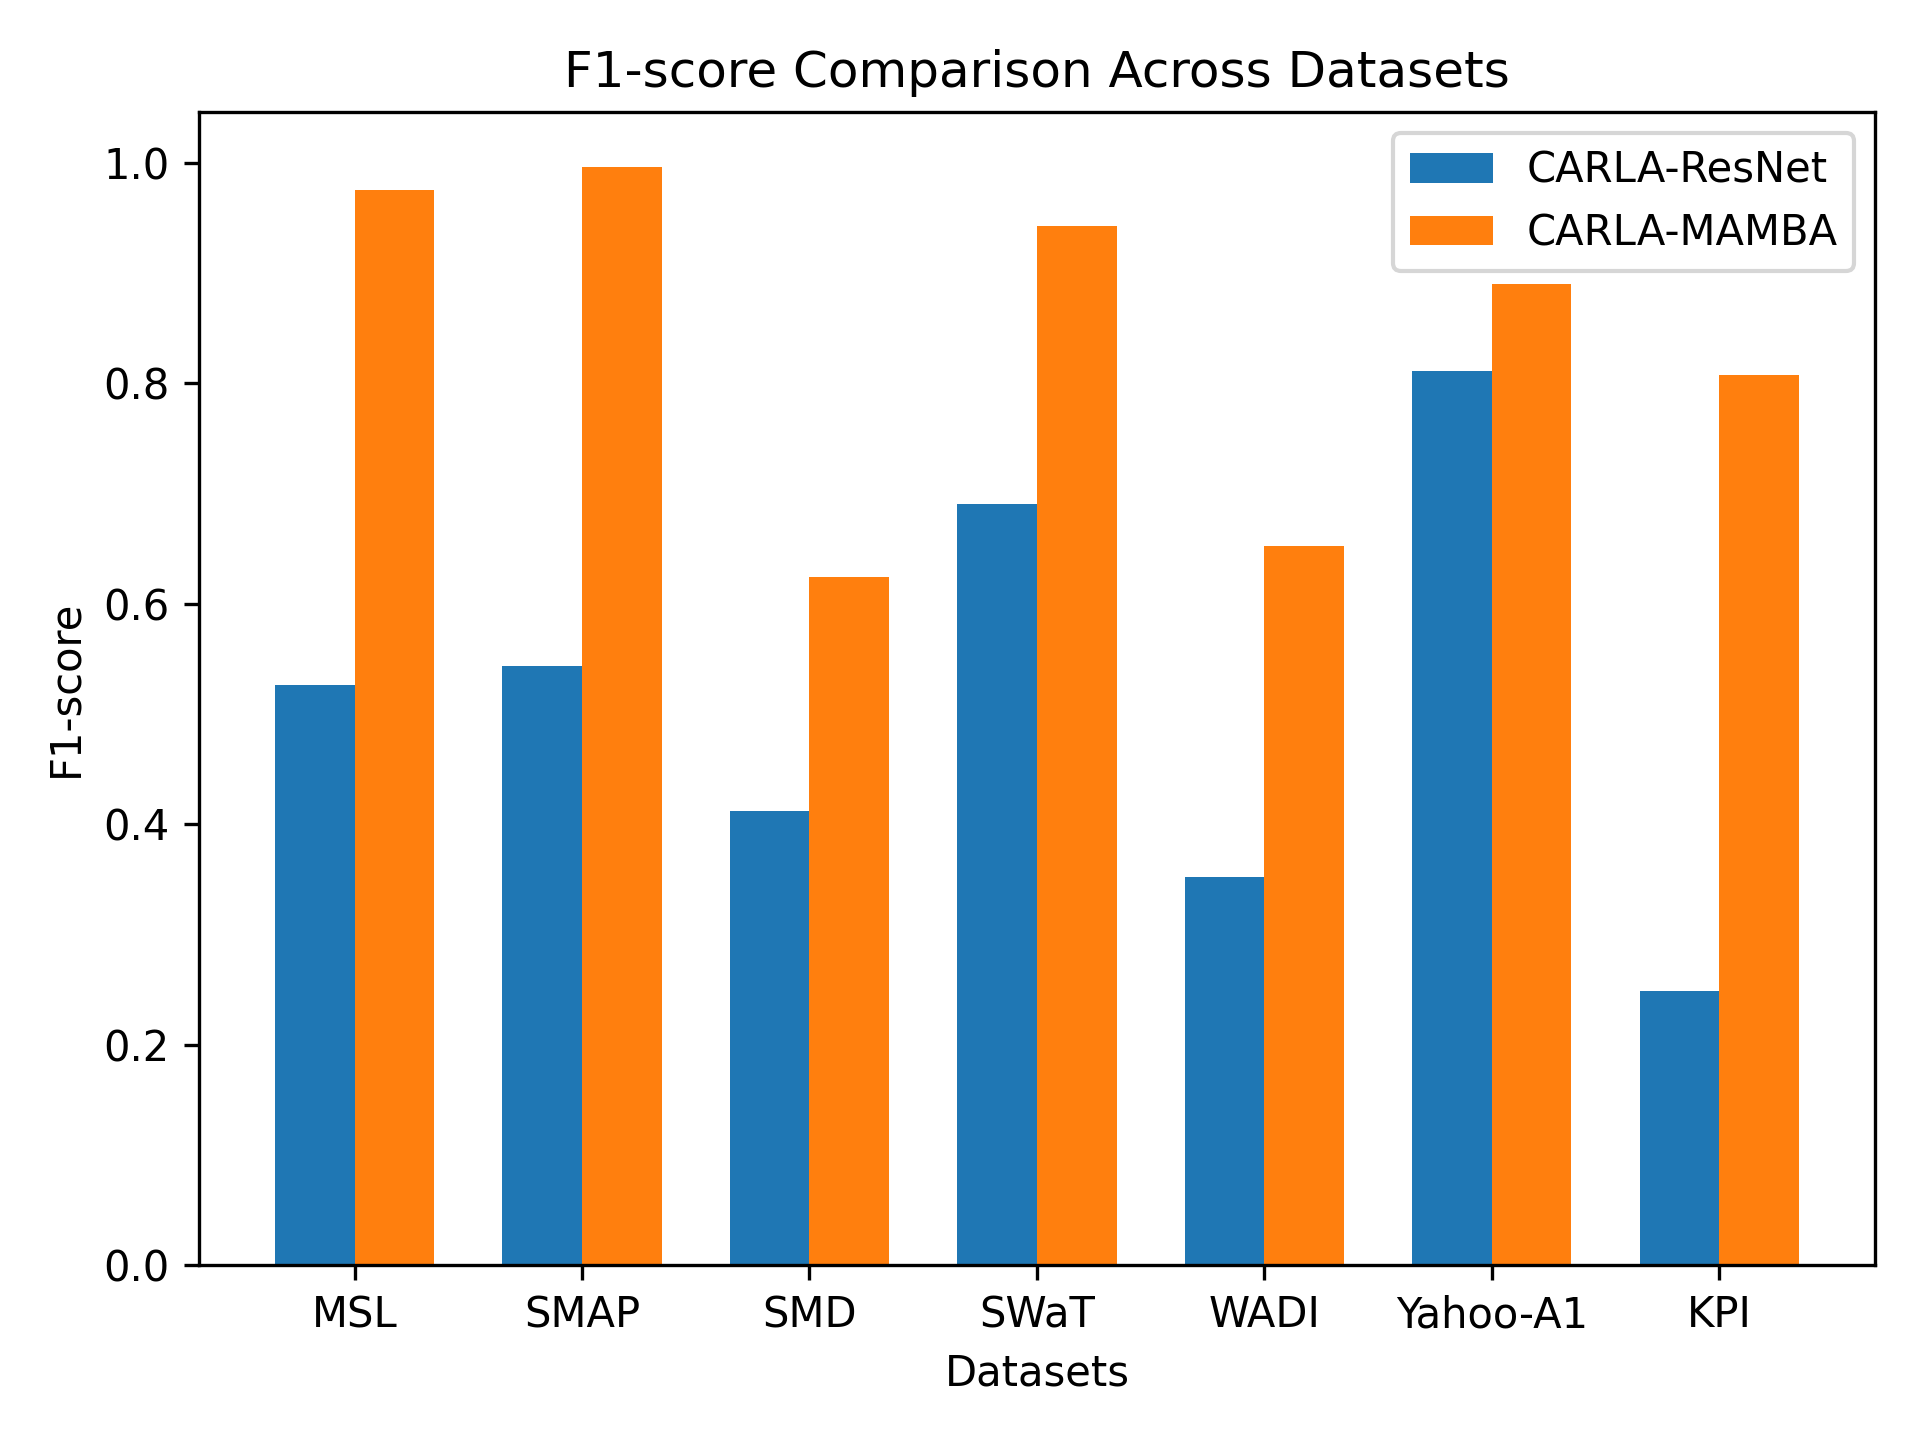
\includegraphics[width=\linewidth]{images/f1_comparison.png}
        \caption{F1-score comparison}
        \label{fig:f1_comparison}
    \end{subfigure}
    \hfill
    \begin{subfigure}[t]{0.48\linewidth}
        \centering
        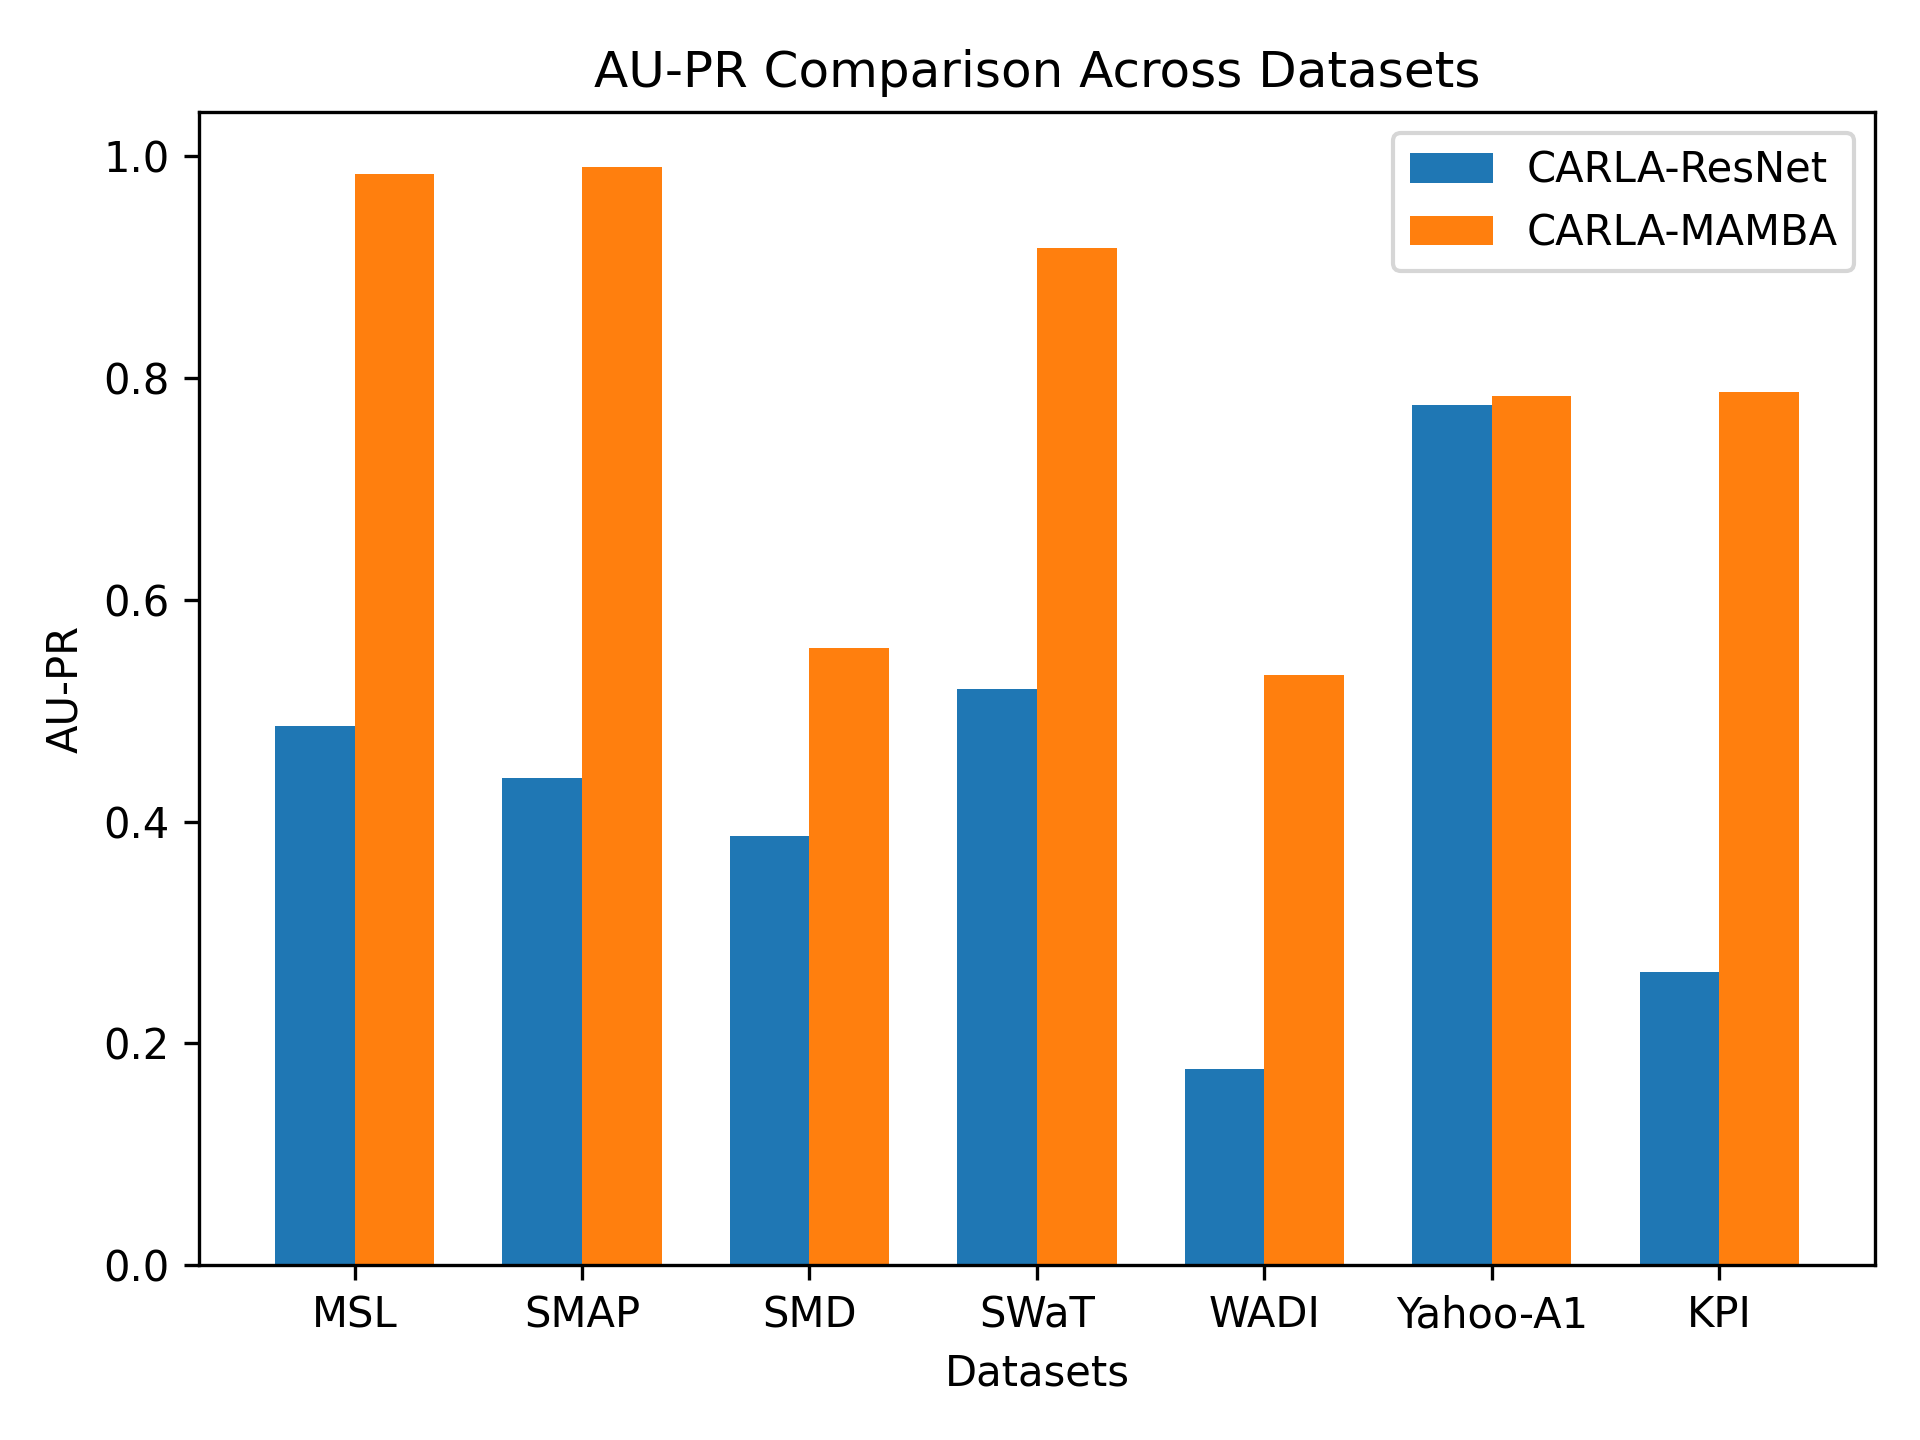
\includegraphics[width=\linewidth]{images/aupr_comparison.png}
        \caption{AU-PR comparison}
        \label{fig:aupr_comparison}
    \end{subfigure}
    
    \caption{Comparison between CARLA-ResNet and CARLA-MAMBA across seven benchmark datasets.}
    \label{fig:combined_results}
\end{figure}

Figure~\ref{fig:combined_results} shows the overall comparison between CARLA-ResNet and CARLA-MAMBA. 
Using the optimal window size for each dataset, CARLA-MAMBA consistently achieves better performance than the original CARLA baseline on all seven datasets in both F1-score and AU-PR.

\subsection{Overall Performance}

Table~\ref{tab:carla_comparison} presents the final comparison between CARLA-ResNet and CARLA-MAMBA using the best window size for each dataset.

CARLA-MAMBA consistently outperforms the original CARLA baseline on all seven benchmark datasets in both F1-score and AU-PR. The improvements are especially large on datasets with long temporal structures.

The largest improvement appears on SMAP, where the F1-score increases from $0.5435$ to $0.9961$, while AU-PR improves from $0.4396$ to $0.9905$. Similar improvements are observed on MSL, where the F1-score increases from $0.5258$ to $0.9750$ and AU-PR improves from $0.4866$ to $0.9838$.

Large F1-score improvements are also observed on KPI ($0.2483 \rightarrow 0.8078$), WADI ($0.3525 \rightarrow 0.6523$), SWaT ($0.6908 \rightarrow 0.9423$), SMD ($0.4123 \rightarrow 0.6242$), and Yahoo-A1 ($0.8111 \rightarrow 0.8897$).

These results reveal an important trend. Mamba achieves its strongest improvements when the window size is sufficiently large to capture long-range temporal dependencies. In earlier experiments using smaller windows, Mamba often underperformed because the temporal context was too limited. After increasing the window size appropriately for each dataset, the performance improves dramatically across all benchmarks.

This finding suggests that the effectiveness of Mamba in time-series anomaly detection depends strongly on matching the window size to the temporal structure of the dataset.

\begin{table}[htbp]
\centering
\caption{Final comparison between CARLA-ResNet and CARLA-MAMBA using the best window size for each dataset.}
\label{tab:carla_comparison}
\resizebox{\linewidth}{!}{
\begin{tabular}{llccccccc}
\hline
\textbf{Dataset} & \textbf{Method} &
\textbf{Prec} & \textbf{Rec} & \textbf{F1} & \textbf{AU-PR} &
\textbf{Time (s)} & \textbf{Avg./Series (s)} & \textbf{Mem.(MB)} \\
\hline

\multirow{2}{*}{MSL}
& ResNet & 0.3910 & 0.8025 & 0.5258 & 0.4866 $\pm$ 0.2519 & 12351.98 & 457.48 & 1230.80 \\
& MAMBA & \textbf{0.9630} & \textbf{0.9873} & \textbf{0.9750} & \textbf{0.9838 $\pm$ 0.0469} & 5598.14 & 207.34 & 6859.53 \\
\hline

\multirow{2}{*}{SMAP}
& ResNet & 0.4233 & 0.7589 & 0.5435 & 0.4396 $\pm$ 0.3217 & 33924.34 & 616.81 & 382.69 \\
& MAMBA & \textbf{0.9923} & \textbf{1.0000} & \textbf{0.9961} & \textbf{0.9905 $\pm$ 0.0676} & 14015.99 & 254.84 & 1176.30 \\
\hline

\multirow{2}{*}{SMD}
& ResNet & 0.3144 & 0.5987 & 0.4123 & 0.3870 $\pm$ 0.1908 & 33763.76 & 1205.85 & 1540.48 \\
& MAMBA & \textbf{0.4835} & \textbf{0.8804} & \textbf{0.6242} & \textbf{0.5564 $\pm$ 0.1856} & 35260.63 & 1259.31 & 5926.61 \\
\hline

\multirow{2}{*}{SWaT}
& ResNet & 0.7917 & 0.6126 & 0.6908 & 0.5193 & 1142.35 & 1142.35 & 206.96 \\
& MAMBA & \textbf{1.0000} & \textbf{0.8909} & \textbf{0.9423} & \textbf{0.9175} & 1190.11 & 1190.11 & 623.77 \\
\hline

\multirow{2}{*}{WADI}
& ResNet & 0.2202 & 0.8824 & 0.3525 & 0.1771 & 1496.77 & 1496.77 & 179.48 \\
& MAMBA & \textbf{0.4840} & \textbf{1.0000} & \textbf{0.6523} & \textbf{0.5322} & 2877.58 & 2877.58 & 1127.98 \\
\hline

\multirow{2}{*}{Yahoo-A1}
& ResNet & 0.6946 & 0.9746 & 0.8111 & 0.7761 $\pm$ 0.3397 & 5609.75 & 102.00 & 42.39 \\
& MAMBA & \textbf{0.8047} & \textbf{0.9948} & \textbf{0.8897} & \textbf{0.7835 $\pm$ 0.3677} & 3444.70 & 62.63 & 165.87 \\
\hline

\multirow{2}{*}{KPI}
& ResNet & 0.1500 & 0.7206 & 0.2483 & 0.2644 $\pm$ 0.2343 & 62356.69 & 2150.23 & 371.06 \\
& MAMBA & \textbf{0.6887} & \textbf{0.9768} & \textbf{0.8078} & \textbf{0.7879 $\pm$ 0.2227} & 80907.62 & 2789.92 & 1715.25 \\
\hline

\end{tabular}
}
\end{table}

\subsection{Inference Time and Memory}

The experimental results also reveal several important trends regarding computational efficiency and GPU memory usage.

On MSL, SMAP, and Yahoo-A1, CARLA-MAMBA is substantially faster than the ResNet baseline after using larger windows. For example, on SMAP, the total inference time decreases from $33924.34$ seconds to $14015.99$ seconds. Similarly, on MSL, the inference time decreases from $12351.98$ seconds to $5598.14$ seconds.

This improvement occurs because larger windows reduce the total number of sliding windows processed during inference. Since Mamba can efficiently model long sequences using its selective state space mechanism and parallel scan algorithm, increasing the window size reduces redundant computations across overlapping windows.

However, larger windows also increase GPU memory usage. On MSL, GPU memory increases from $1230.80$ MB to $6859.53$ MB. Similar increases appear on SMD and WADI. Several larger configurations could not be evaluated because they exceeded the 16 GB memory limit of the Tesla T4 GPU.

These observations show an important trade-off in CARLA-MAMBA. Larger windows often improve anomaly detection performance and reduce inference time, but they also require significantly more GPU memory.

% ---- Discussion ----
\section{Discussion}

\subsection{Effect of Window Size on Mamba}

One of the most important findings of this work is that Mamba performance scales strongly with temporal context when the anomaly structure requires long-range dependency modeling.

For short-series datasets such as SMAP and MSL, increasing the window size produces almost monotonic improvements in both F1-score and AU-PR until a saturation point is reached. This behavior indicates that Mamba benefits substantially from observing broader temporal context and can effectively utilize long-range sequential information.

In contrast, datasets containing highly localized anomalies exhibit different behavior. On SWaT, performance decreases significantly when the window becomes excessively large. This suggests that overly broad temporal context may dilute sharp anomaly patterns by mixing them with dominant normal regions.

These observations indicate that the optimal window size depends not only on sequence length but also on anomaly locality. Long-range anomaly structures favor large windows, whereas localized anomaly patterns prefer compact temporal context.

\subsection{Why Mamba Improves CARLA}

The results show that replacing the ResNet backbone with Mamba substantially improves the quality of learned representations in the CARLA framework.

The original ResNet backbone mainly captures local temporal patterns through small convolution kernels. While this is effective for short local anomalies, it limits the ability to model long-range dependencies across large temporal intervals.

In contrast, Mamba processes the full sequence using a selective state space mechanism. This allows the encoder to dynamically decide which temporal information should be preserved or ignored at each time step. As a result, the learned representations contain richer temporal structure and better separate normal and anomalous patterns.

The improvement is especially large on datasets with long sequences such as MSL, SMAP, and KPI. These datasets require modeling information across very large temporal ranges, which is difficult for convolution-based encoders.

The results also suggest that the quality of the pretext representations is highly important for the second classification stage in CARLA. Better embeddings lead to more accurate nearest-neighbor relationships, which improves the final anomaly classification boundaries.

\subsection{Trade-off Between Performance and Memory}

Although large windows improve anomaly detection performance substantially, they also lead to much higher GPU memory usage. This trade-off becomes especially important for Mamba-based models because the internal state must be maintained across the entire sequence. As the window size increases, the amount of intermediate state information stored during computation also grows significantly.

This effect can be clearly observed in our experiments. On MSL, the best-performing configuration uses a window size of 2048 and requires more than 6.8 GB of GPU memory, compared to only 1.2 GB for the original ResNet baseline. Similar behavior appears on SMD and WADI, where larger windows produce better F1-scores but also greatly increase memory consumption. For SMD and KPI, some larger window configurations could not be evaluated because they exceeded the 16 GB memory limit of the Tesla T4 GPU.

At the same time, larger windows can also reduce inference time. Since each sliding window covers a broader temporal range, the total number of windows processed becomes smaller. This reduces redundant computation across overlapping windows and can make inference faster despite the higher memory usage. For example, on MSL, increasing the window size from 200 to 2048 reduces the total inference time from 12351.98 seconds to 5598.14 seconds.

These observations show that practical deployment of CARLA-MAMBA requires balancing anomaly detection performance, inference efficiency, and hardware memory constraints. In practice, the optimal window size is often the largest value that still fits within the available GPU memory budget.

\subsection{Limitations}

This work has several limitations.

First, the experiments are constrained by the 16 GB memory capacity of the Tesla T4 GPU. Several potentially beneficial large-window configurations could not be evaluated because they exceeded the available hardware memory.

Second, the experiments were conducted using a single random seed. Evaluating multiple seeds would provide stronger statistical reliability.

Third, although we propose a practical heuristic for window size selection based on sequence length and GPU constraints, the strategy still requires limited empirical validation for new datasets, especially when anomaly locality characteristics are unknown.

Finally, the current study focuses only on replacing the stage-1 ResNet encoder in CARLA with Mamba. Exploring hybrid architectures and replacing both stages simultaneously may further improve representation quality and detection performance.

% ---- Conclusion ----
\section{Conclusion and Future Work}

In this paper, we proposed CARLA-MAMBA, a modified version of the CARLA framework where the ResNet backbone in the pretext stage is replaced with Mamba, a selective state space model designed for efficient long-sequence modeling.

We conducted extensive experiments on seven benchmark datasets and performed systematic window size ablation studies. The results show that window size is a critical factor for Mamba-based time-series anomaly detection.

When the temporal window is properly selected, CARLA-MAMBA consistently outperforms the original CARLA baseline across all seven benchmark datasets in both F1-score and AU-PR.

Our experiments also reveal a strong relationship between dataset characteristics and optimal window size. Datasets with long temporal dependencies benefit significantly from large windows, while datasets with highly local anomalies prefer smaller temporal context.

These findings demonstrate that Mamba is a highly effective backbone for self-supervised time-series anomaly detection when sufficient temporal context is available.

Future work will focus on developing theoretically grounded automatic window selection methods, memory-efficient long-sequence training strategies, and hybrid architectures that combine local convolutional modeling with global state space modeling. We also plan to investigate newer selective state space models such as Mamba-2 and multi-stage sequence modeling architectures for anomaly detection.

\section*{Declaration of competing interest}
Declaration of generative AI and AI-assisted technologies in the writing process ChatGPT was used for assisting with language editing only. The authors reviewed and revised the manuscript and take full responsibility for the accuracy and integrity of the work.
% ---- Bibliography ----
\bibliographystyle{splncs03_unsrt}
\bibliography{references}

\end{document}